\begin{figure}[h]
\centering
% TransE diagram
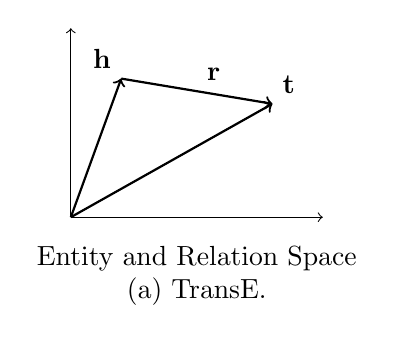
\begin{tikzpicture}[scale=0.8]
\label{subfig:transE}
    % Coordinate system
    \draw[->] (0,0) -- (4,0);
    \draw[->] (0,0) -- (0,3);
    
    % Points
    \coordinate (O) at (0,0);
    \coordinate (h) at (0.8,2.2);
    \coordinate (t) at (3.2,1.8);
    \coordinate (r_start) at (4.8,3);
    
    % Vectors
    \draw[->, thick] (O) -- (h) node[above left] {$\mathbf{h}$};
    \draw[->, thick] (O) -- (t) node[above right] {$\mathbf{t}$};
    \draw[->, thick] (h) -- (t) node[midway, above right] {$\mathbf{r}$};
    
    % Labels
    \node[below] at (2,-0.3) {Entity and Relation Space};
    \node[below] at (2,-0.8) {(a) TransE.};
\end{tikzpicture}
\hspace{1cm}
% TransH diagram
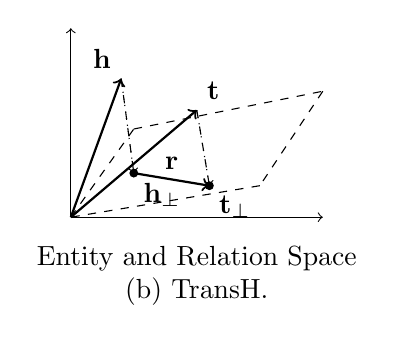
\begin{tikzpicture}[scale=0.8]
\label{subfig:transH}
    % Coordinate system
    \draw[->] (0,0) -- (4,0);
    \draw[->] (0,0) -- (0,3);
    % Hyperplane coords
    \coordinate (h1) at (0,0);
    \coordinate (h2) at (1,1.4);
    \coordinate (h3) at (4,2);
    \coordinate (h4) at (3,0.5);
    
    % Hyperplane (dashed line)
    \draw[dashed] (h1) -- (h2);
    \draw[dashed] (h2) -- (h3);
    \draw[dashed] (h3) -- (h4);
    \draw[dashed] (h4) -- (h1);
    
    % Points
    \coordinate (O) at (0,0);
    \coordinate (h) at (0.8,2.2);
    \coordinate (t) at (2,1.7);
    \coordinate (h_proj) at (1,0.7);
    \coordinate (t_proj) at (2.2,0.5);
    
    % Original vectors
    \draw[->, thick] (O) -- (h) node[above left] {$\mathbf{h}$};
    \draw[->, thick] (O) -- (t) node[above right] {$\mathbf{t}$};
    % Relation vector
    \draw[->, thick] (h_proj) -- (t_proj) node[midway, above] {$\mathbf{r}$};
    
    % Projected vectors
    \draw[->, dashed] (h) -- (h_proj) node[below right] {$\mathbf{h}_{\perp}$};
    \draw[->, dashed] (t) -- (t_proj) node[below right] {$\mathbf{t}_{\perp}$};
    
    % Projection lines
    \draw[dotted] (h) -- (h_proj);
    \draw[dotted] (t) -- (t_proj);
    % Points at projections
    \fill (h_proj) circle (2pt);
    \fill (t_proj) circle (2pt);
    
    % Labels
    \node[below] at (2,-0.3) {Entity and Relation Space};
    \node[below] at (2,-0.8) {(b) TransH.};
\end{tikzpicture}
\vspace{0.5cm}
% TransR diagram - Combined Entity and Relation Space
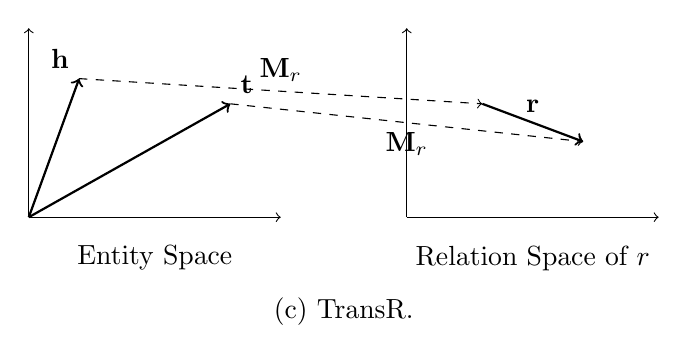
\begin{tikzpicture}[scale=0.8]
\label{subfig:transR}
    % Entity Space (left side)
    % Coordinate system
    \draw[->] (0,0) -- (4,0);
    \draw[->] (0,0) -- (0,3);
    
    % Points in entity space
    \coordinate (O1) at (0,0);
    \coordinate (h) at (0.8,2.2);
    \coordinate (t) at (3.2,1.8);
    
    % Vectors in entity space
    \draw[->, thick] (O1) -- (h) node[above left] {$\mathbf{h}$};
    \draw[->, thick] (O1) -- (t) node[above right] {$\mathbf{t}$};
    
    % Entity space label
    \node[below] at (2,-0.3) {Entity Space};
    
    % Relation Space (right side)
    % Coordinate system
    \draw[->] (6,0) -- (10,0);
    \draw[->] (6,0) -- (6,3);
    
    % Points in relation space
    \coordinate (O2) at (6,0);
    \coordinate (h_r) at (7.2,1.8);
    \coordinate (t_r) at (8.8,1.2);
    
    % Vectors in relation space
    % \draw[->, thick] (O2) -- (h_r) node[above left] {$\mathbf{h}_r$};
    % \draw[->, thick] (O2) -- (t_r) node[above right] {$\mathbf{t}_r$};
    \draw[->, thick] (h_r) -- (t_r) node[midway, above] {$\mathbf{r}$};
    
    % Relation space label
    \node[below] at (8,-0.3) {Relation Space of $r$};
    
    % Matrix transformation arrows connecting the spaces
    \draw[dashed, ->] (h) -- (h_r) node[midway, above] {$\mathbf{M}_r$};
    \draw[dashed, ->] (t) -- (t_r) node[midway, below] {$\mathbf{M}_r$};
    \vspace{0.3cm}
    \node at (5,-1.5) {(c) TransR.};
\end{tikzpicture}
\caption{Illustrations of translation distance models TransE, TransH, and TransR \parencite{ZHANG2024123876}.}
\label{fig:translation_distance_models}
\end{figure}